\chapter{Recetas}
En este capítulo se detallará todo lo relativo al \href{https://github.com/Slowmybrosh/TFG-DietPlanner/milestone/3}{milestone} ``Encontrar recetas'', que tiene como objetivo solucionar al usuario la necesidad de encontrar recetas utilizando exclusivamente los ingredientes seleccionados por el usuario.

\section{Fuente de recetas}
Para la obtención de recetas, se obtendrán de la famosa página de recetas \href{https://cookpad.com/es/home}{Cookpad}. Donde la comunidad puede subir cualquier receta. Habiendo mucha variedad de recetas, permitiendo obtener una base de datos variada. Estas recetas se deberán cargar en una base de datos.

El robot de BluePrism, utiliza un reconocimiento del código fuente, similar a un crawler, de la página permitiendo seleccionar los elementos deseados de cada una. Inspeccionando la página se pueden analizar una serie de atributos para identificar inequívocamente algunos elementos.

Los pasos que se han seguido para obtener recetas son:
\begin{enumerate}
    \item Buscar diferentes recetas de diferentes tipos (pescado, carne, verduras, etc...)
    \item Obtener los enlaces de dichas recetas
    \item Filtrar los enlaces para evitar los repetidos
    \item Acceder a cada receta y recuperar
    \begin{enumerate}
        \item Nombre
        \item Ingredientes
        \item Pasos
    \end{enumerate}
    \item Formar un fichero en formato JSON
\end{enumerate}

Para la función de buscar recetas de diferentes tipos, se lanza un navegador web con la dirección de inicio de \href{https://cookpad.com/es/home}{Cookpad}, al buscar cualquier cosa utilizando el cuadro de búsqueda. La dirección a la que se consulta la petición es la siguiente: https://cookpad.com/es/buscar/verduras?event=search.history&order=recent, con un simple vistazo se puede identificar que la petición en este caso fue ``verduras''. Sabiendo esto, para buscar por tipo de receta se han compuesto las direcciones url de manera dinámica, evitando pasos extra a la hora de realizar esta búsqueda inicial. 

\begin{figure}[h!]
    \centering
    \fbox{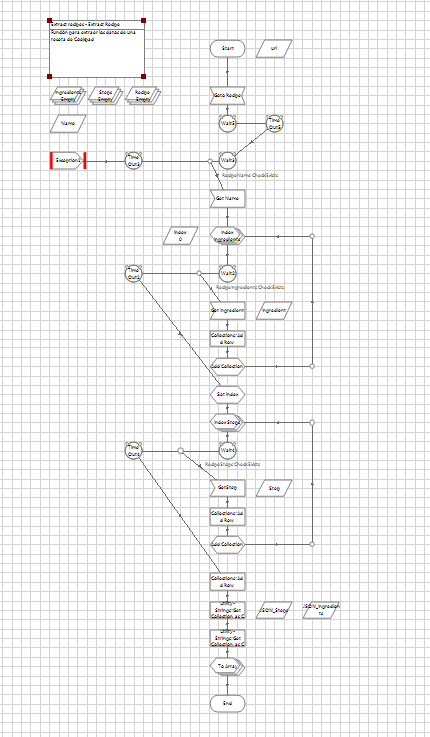
\includegraphics[width=100mm,scale=1]{./images/Extract_recipe.png}}
    \caption{Función para extraer enlaces}
    \label{fig:links}
\end{figure}

En el paso de obtención de la receta, se identifica el nombre de la receta. Utilizando la herramienta de modelado de aplicación que trae incorporada BluePrism. Con ella se puede seleccionar el elemento de la página que se desea extraer y automáticamente se extrae información relevante para la identificación como el identificador del elemento, las clases CSS del mismo, su ruta XPATH, etc... El nombre de las recetas como elemento no es único, al ser una lista de recetas habrá muchas coincidencias que se quieran extraer. Para ello se utiliza el atributo \emph{match_index}, si se selecciona el primer resultado de la página se obtendría el primer nombre. BluePrism permite recuperar atributos dinámicos, en la función el número de coincidencia itera entre uno y diez para obtener diez recetas de cada tipo. Con la coincidencia del elemento, se extrae el enlace y se guarda en una colección que se pasará a la función para extraer recetas. 

\begin{figure}[h!]
    \centering
    \fbox{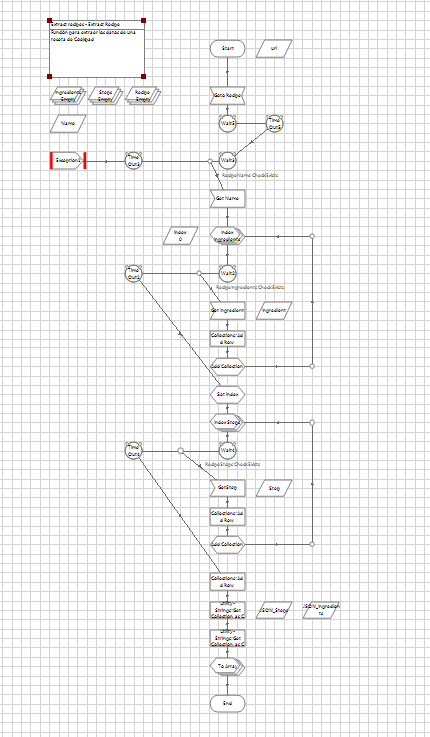
\includegraphics[width=100mm,scale=1]{./images/Extract_recipe.png}}
    \caption{Función para extraer recetas}
    \label{fig:links}
\end{figure}

Una vez obtenidos todos los enlaces, puede que haya repetidos por coincidir en la categoría de carne y verduras a la vez, es necesario hacer un filtrado muy sencillo que elimine los enlaces repetidos. 

La función que extrae la receta de la página, obtiene el nombre teniendo en cuenta que es el primer \emph{h1} de la página. Los ingredientes y los pasos se tratan de listas ordenadas, fáciles de extraer. Cada ingrediente tienen un identificador \emph{ingredient} seguido de una cadena de números. BluePrism puede utilizar \emph{wildcards} para identificar elementos de la página web, de la misma manera que al extraer una lista de enlaces, se itera por los ingredientes hasta que no haya más. Con los pasos se sigue el mismo razonamiento, valiéndose de un selector CSS para extraer los pasos iterando sobre ellos hasta que no hay más. 

\begin{figure}[h!]
    \centering
    \fbox{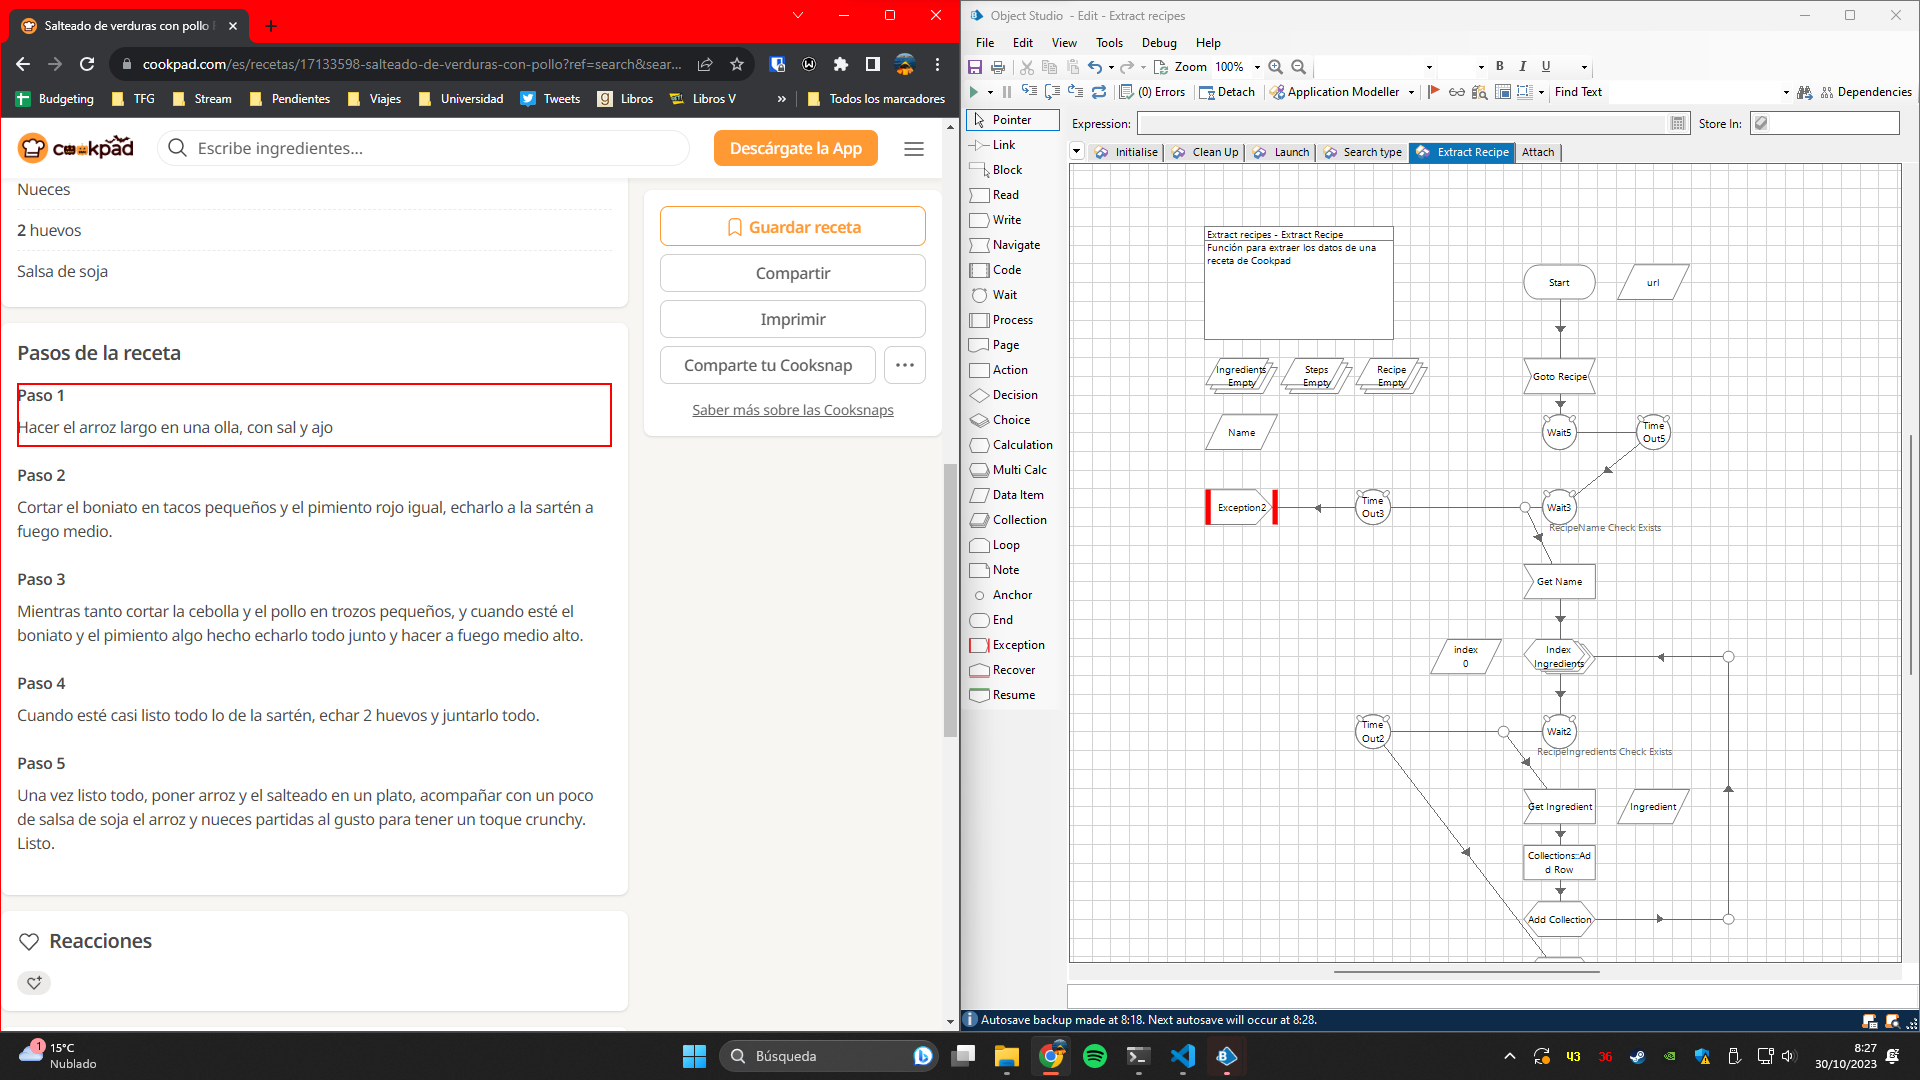
\includegraphics[width=100mm,scale=1]{./images/identify_step.png}}
    \caption{Identificar los pasos de la receta}
    \label{fig:links}
\end{figure}


Para que constituya una fuente de información uniforme, la colección de recetas se guarda como un fichero JSON que puede ser fácilmente recuperado y transformado en cualquier otro formato.

El proceso de ejecución del robot lleva tiempo, ya que el identificar los ingredientes a través de una expresión regular toma entre diez y veinte segundos. Los demás pasos son relativamente menos costosos en cuestión de tiempo. El robot tardó aproximadamente cuatro horas en obtener sesenta y dos recetas con todos los elementos mencionados. La ventaja de haber utilizado este proceso de obtención de recetas es que se puede ampliar en el futuro a conveniencia, aunque hay que tener en cuenta el tiempo que tarda el robot en obtener recetas.